\subsection{Product perspective}
\subsubsection{Class diagram}
This section will present the high-level UML class diagrams of the application.
\\\\
\begin{figure}[H]
    \centering
    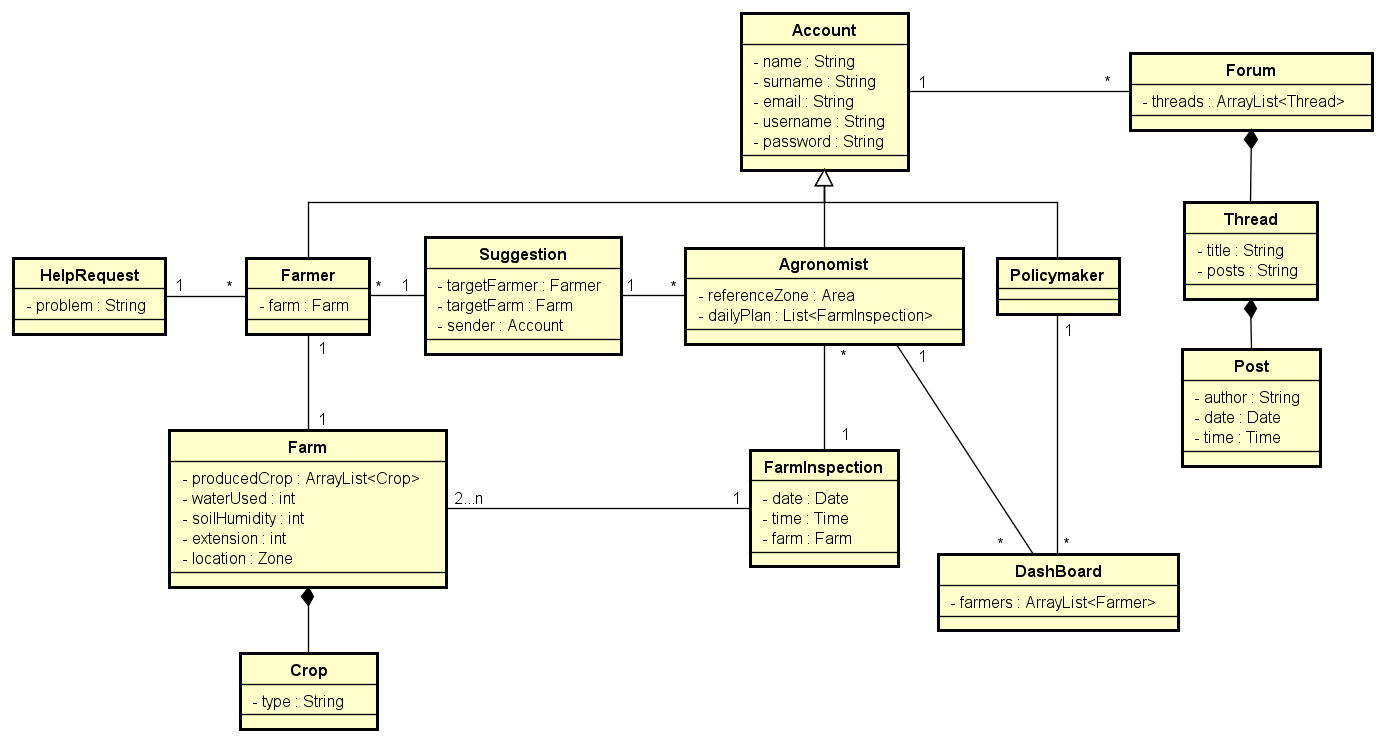
\includegraphics[width=\textwidth,height=\textheight,keepaspectratio]{Images/HighLevelUMLcut.png}
    \caption{\label{fig:high_level_uml}High level class diagram}
\end{figure}

\bigskip
\paragraph{Additional notes on the class diagram}
\begin{itemize}
    \item The agronomist attribute dailyPlan is a collection of FarmInspection ordered by date and time
    \item Agronomists can create a suggestion responding to a farmer help request
\end{itemize}

\newpage
\subsubsection{State machine diagrams}
The following diagrams are meant to give a high-level description of the states' evolution during the system processes.
\\\\

\begin{figure}[H]
    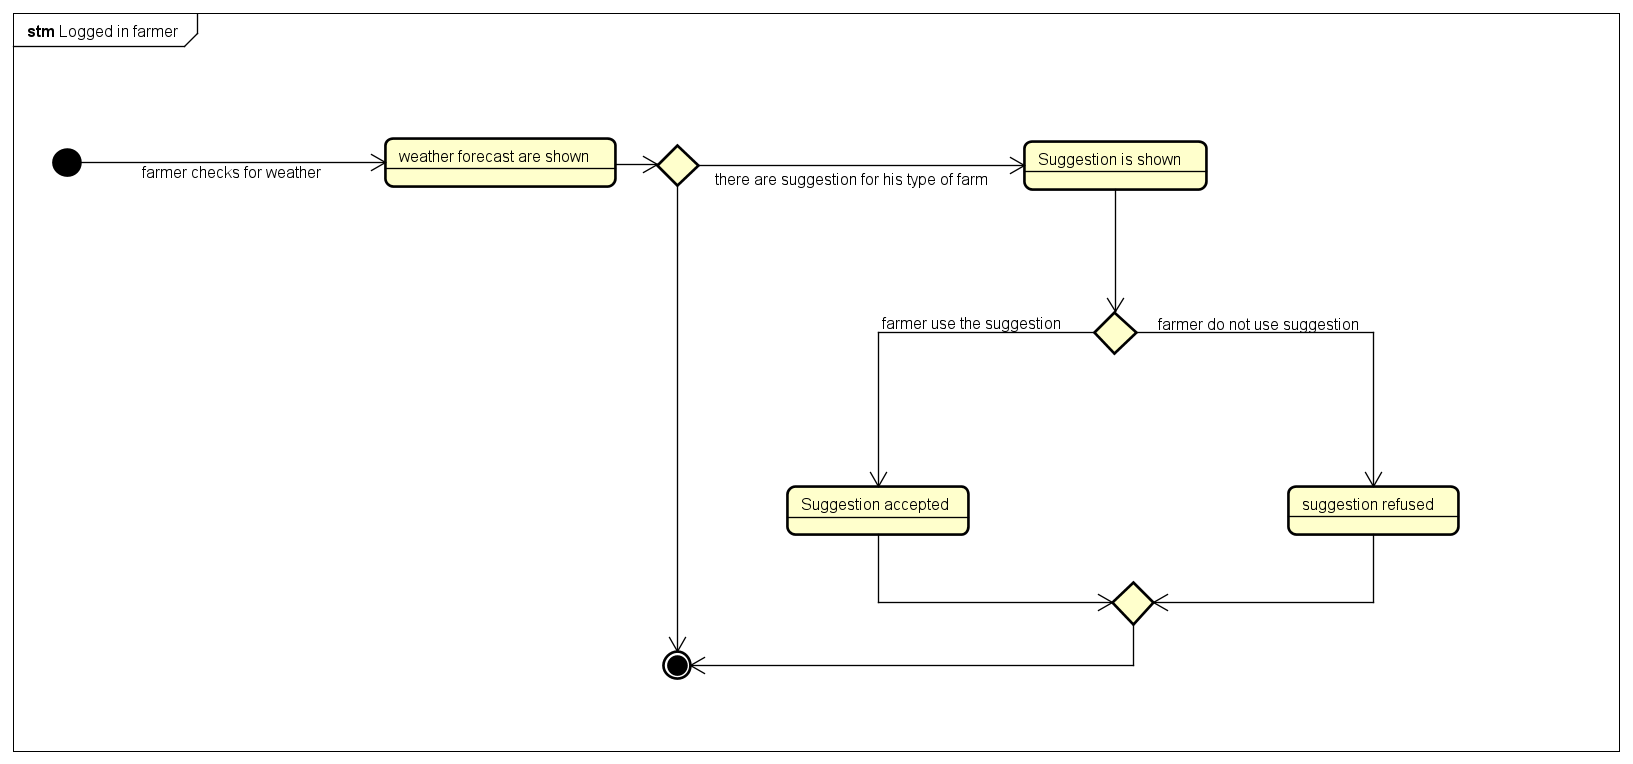
\includegraphics[width=\textwidth,height=\textheight,keepaspectratio]{Images/farmerChecksWeather.png}
    \caption{Statechart of a farmer checking weather forecast}
    \label{fig:statechart_farmer_weather}
\end{figure}

\begin{figure}[H]
    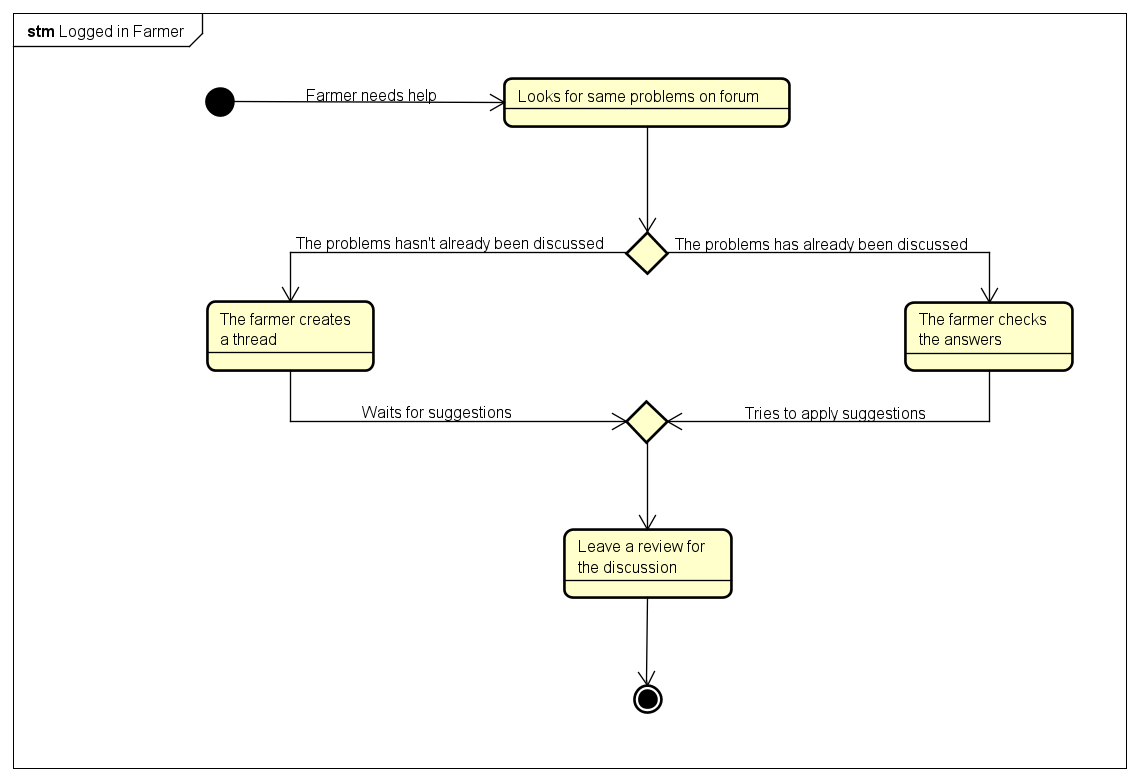
\includegraphics[width=\textwidth,height=\textheight,keepaspectratio]{Images/farmerCreatesThread.png}
    \caption{Statechart of the lifetime of a discussion thread on the forum}
    \label{fig:statechart_farmer_thread}
\end{figure}

\begin{figure}[H]
    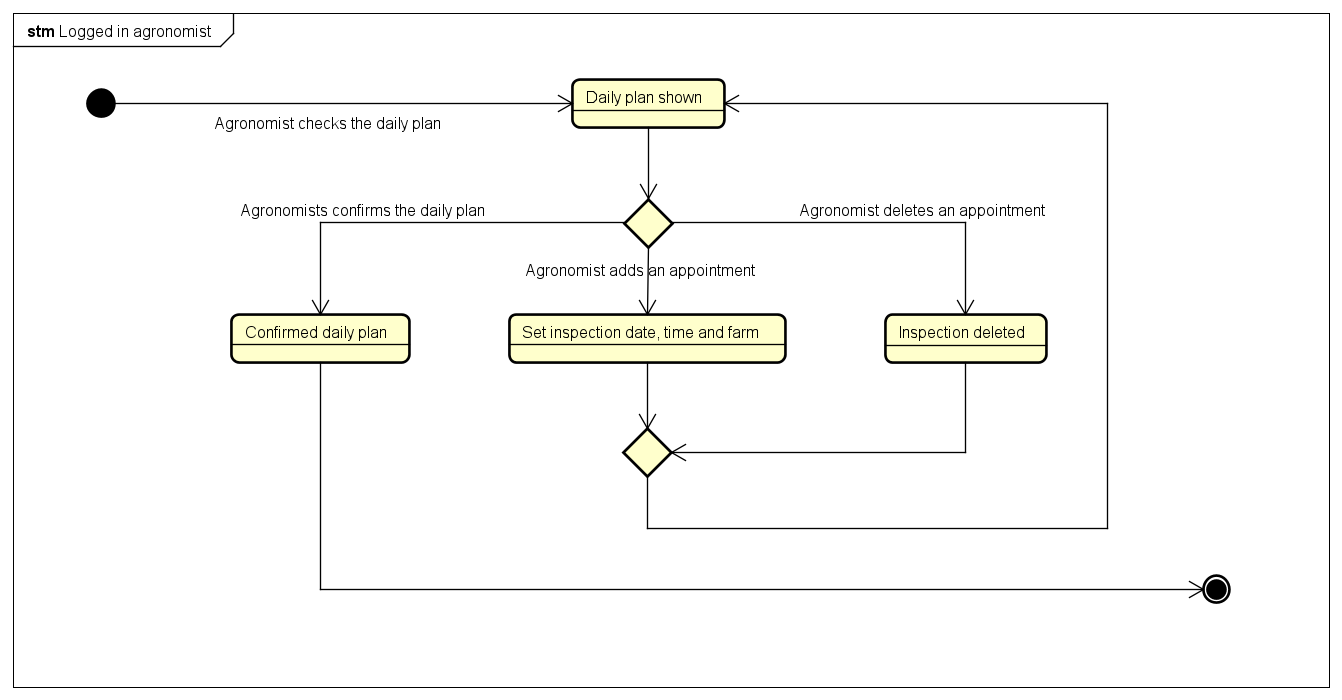
\includegraphics[width=\textwidth,height=\textheight,keepaspectratio]{Images/agronomistDailyPlan.png}
    \caption{Statechart of an agronomist managing his daily plan}
    \label{fig:statechart_agronomist_plan}
\end{figure}

\bigskip
\begin{figure}[H]
    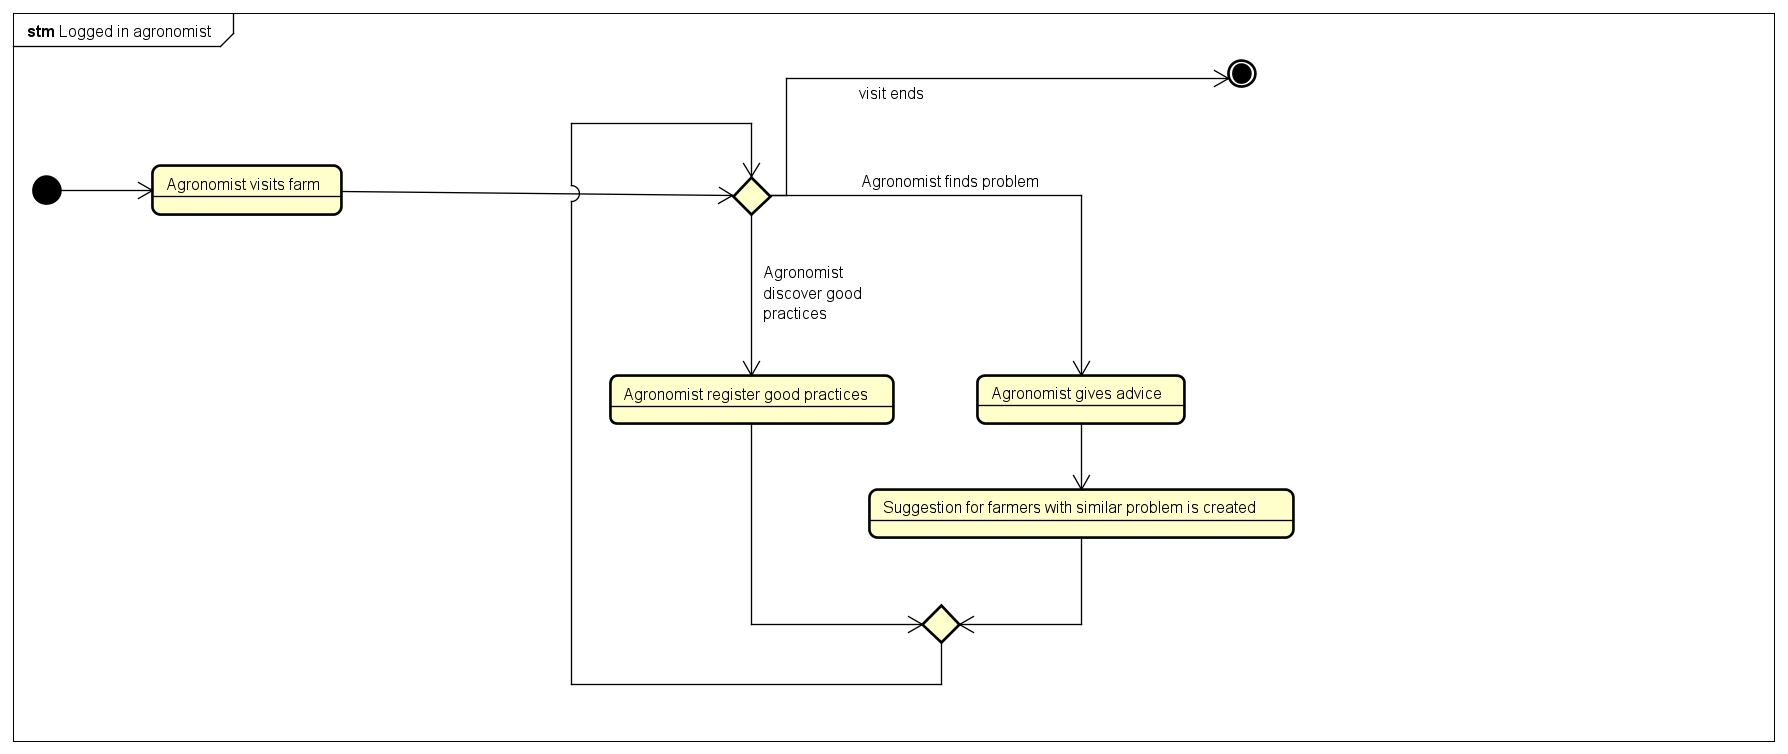
\includegraphics[width=\textwidth,height=\textheight,keepaspectratio]{Images/agronomistVisitFarm.png}
    \caption{Statechart of the lifetime of a farm visit}
    \label{fig:statechart_agronomist_visit}
\end{figure}

\newpage
\subsection{Product functions}
\emph{DREAM} offers Farmers the ability to ask for help from other farmers or an agronomist, 
they can check the weather forecast and see if there are suggestions for them. 
\emph{DREAM} create a dashboard with information about farmers that both agronomist and policymakers can
visualize. The first ones can set thresholds and both can visualize data concerning the agricultural production of Telangana.
Especially they can discover which farmers overcame thresholds, and the performance of farmers who received help.
In addition, \emph{DREAM} offers agronomists the possibility of visualizing, modifying or confirming their daily plan.

\paragraph{Common user functions} These functions are available to all Users:
\begin{itemize}
    \item \textbf{Registration and Login}\\
          Users should be able to create an account on the App using personal email and password.
          In this process, he has to select his role.
          \newline By logging in with their account, users can access the other functions.
\end{itemize}

\paragraph{Basic Farmer functions} These functions are available to all logged-in Farmers:
\begin{itemize}
    \item \textbf{Check weather forecast}\\
          \emph{DREAM} retrieves meteorological short-term and long-term data from an external source and makes them available 
          to farmers. They can check the forecasts on the app and if there are suggestions for their farm these are shown to them.
           These suggestions are created when an agronomist helps a farmer in a similar situation.
    \item \textbf{Request help}\\
          A farmer in case of a problem can ask for the direct help of an agronomist. He can use a section to send a help request,
           when this functionality is used a notification is sent to the agronomist responsible for the location of the farm with informations about the problem and the farm.
    \item \textbf{Create discussion on forum}\\
         \emph{DREAM} has a forum section on which farmers can create a discussion specifying the type of problem and eventual specificity of their farm. 
    \item \textbf{Reply to forum discussion}
        After access to the forum section of \emph{DREAM}, the farmer can select a recent, not closed discussion and post a reply.
    \item \textbf{Close a discussion}
        A farmer after receiving an effective reply can mark the answer as effective and close the discussion.
    \item \textbf{Insert production data}
        A farmer periodically insert in the app the amount of crops produced, the type and the amount of water used.
\end{itemize}

\paragraph{Agronomist base functions}
These functions should be accessible to all logged-in Agronomists
\begin{itemize}
    \item\textbf{Insert area he is responsible for}\\
    From the home page, the agronomist can open a geographical representation of Telangana
    and select the area he is responsible for. \emph{DREAM} checks if the selected territory is already overseen
    by another agronomist. In that case, the app asks the user to repeat the process;
    otherwise, the selection is saved on \emph{DREAM}'s database.
    \item \textbf{Reply to forum discussion}\\
    After access to the forum section of \emph{DREAM}, the agronomist can select a recent,
    not closed discussion and post a reply.
    \item \textbf{Reply to help request}\\
    On receiving a private help request from a farmer, the agronomist receives a notification containing the sender
    and the problems they need to face. He can choose between two options: answer the request or plan a visit.
    \item \textbf{Visualize dashboard}\\
    \emph{DREAM} offers the possibility to the agronomist of visualizing the best
    performing farmers in his related area; these farmers are selected through thresholds
    (concerning the production and especially the resilience to meteorological adverse events)
    created by the agronomist of the corresponding area.
    \item\textbf{Daily plan management}\\
    From his personal area, the agronomist can visualize the daily plan on a calendar.
    The user has three possible choices: add or delete an appointment and confirm the plan;
    the first two can be repeated several times until the confirmation. In case of deletion of a visit with a given farmer,
    \emph{DREAM} reinserts automatically the same appointment, according to the agronomist's availability,
    only if with that farmer there are less than two visits planned for that year.
    \newline At the end of each day, the agronomist has to confirm the execution of the daily plan or specify
    the deviations from that.
    \item\textbf{Insert good practices}\\
    The agronomist after the visit to a farm can add good practices
    that will be available to farmers with similar conditions and crops.
    \item \textbf{Check weather forecast}\\
    \emph{DREAM} retrieves meteorological short-term and long-term data from an external source and makes them available
    to agronomists.
\end{itemize}

\paragraph{Basic Policy maker functions} These functions are available to all logged-in Policy makers:
\begin{itemize}
    \item \textbf{Visualize farmers' performance}\\
    DREAM provides policy makers with a dashboard with comprehensive data about farmers in Telangana.
    The dashboard shows farmers who are exceeding the thresholds (those will receive special incentives)
    and who are not.
\end{itemize}

\newpage
\subsection{User characteristics}

DREAM is meant to be accessible for both specialized and unspecialized users.

\paragraph{Users}
\begin{itemize}
    \item \textbf{Farmer}: people that own a farm and may need help
    \item \textbf{Agronomist}: someone who is specialized in agriculture activity and is responsible for a given area
    \item \textbf{Policy maker}: people who oversight the agricultural process of Telangana
\end{itemize}

\bigskip
\subsection{Assumptions, dependencies and constraints}
\begin{description}
    \item[D1] Each user creates only one account
    \item[D2] The information provided by the farmer is correct
    \item[D3] The thresholds provided by the agronomists are reasonable for the zone they are responsible for
    \item[D4] Most of the farmers that receive suggestions will enact them
    \item[D5] The answers to the forum's threads are consistent
    \item[D6] A privately help request to an agronomist is replied
    \item[D7] Users will be instructed to use the application if possible
    \item[D8] Agronomist is entitled to choose only his area of responsibility
    \item[D9] Each area has only one responsible agronomist 
    \item[D10] Each farmer owns only one farm 
\end{description}